\chapter{評価}
\label{chap:evaluation}

本章では、ESP32上に実装した実行環境を用いてWebAssemblyバイナリを実行することで、実行速度やメモリフットプリントを示し、マイコンにおけるWebAssembly実行環境が持つ制約を明らかにする。

\section{評価手法}

計測用のプログラムとして、与えられた整数$n$に対して$n$番目のフィボナッチ数を返す関数$fib(n)$をC言語で実装した。

\begin{itembox}[l]{フィボナッチ関数のC言語による実装}
  \begin{verbatim}
    int fib(int n) {
      if (n <= 1) return 1;
      return fib(n - 1) + fib(n - 2);
    }
  \end{verbatim}
\end{itembox}

この関数をLLVM/Clang 7.0によりコンパイルして、85バイトのWebAssemblyバイナリを得た。
このバイナリを\ref{chap:implementation}章で述べたホストプログラムに埋め込み、libwasmによりパースおよびインスタンス化を行った上で、対応する関数を呼び出した。
また、同じ関数をホストプログラムの一部としてコンパイルし、直接呼び出した。

libwasmによる実行およびネイティブの実行の両方で関数が正しい値を返すことを確認した上で、それぞれの場合において\verb|fib|関数に与える引数\verb|n|を0から13まで変化させ、各\verb|n|ごとの実行速度およびメモリフットプリントを計測し比較した。

\section{実行速度}

実行速度は、ESP-IDFが提供する\verb|esp_timer_get_time|関数を用いて計測した。
ESP-IDFを用いてコンパイルされたプログラムは、起動後\verb|esp_timer_init|関数を自動的に呼び出し、タイマーを初期化する。
\verb|esp_timer_get_time|関数は、このタイマーが初期化されてからの経過時間をマイクロ秒単位で返す。
0から13までの各$n$について、\verb|fib|関数の実行直前および実行直後に\verb|esp_timer_get_time|関数を呼び出し、差分を実行時間とした。

ネイティブ実行に対するWebAssemblyバイナリの実行時間について、引数$n$ごとの推移を図\ref{fig:fib_time}に示す。
横軸はフィボナッチ関数の引数$n$、縦軸は実行時間(マイクロ秒)を対数軸で示した片対数グラフである。

本実装およびネイティブ実行の双方において、定数を返す$n=0$および$n=1$の時は、引数による実行時間の増加がなかった。
定数を返す処理においては、本実装の実行時間はネイティブ実行の約260倍だった。

再帰的な関数呼び出しが発生する$n>2$の場合においては、本実装での実行時間は指数的に上昇した。
ネイティブ実行では$n\le5$の場合において、コンパイラによる最適化のためか実行時間は一定だったが、$n>6$の場合では指数的に上昇した。

図\ref{fig:fib_time_diff}は、$fib(n-1)$の実行時間に対する$fib(n)$の実行時間の割合を示したものである。

(分析と考察)

\begin{figure}[htbp]
  % \begin{minipage}{0.5\hsize}
    \caption{実行時間の変化}
    \label{fig:fib_time}
    \begin{center}
      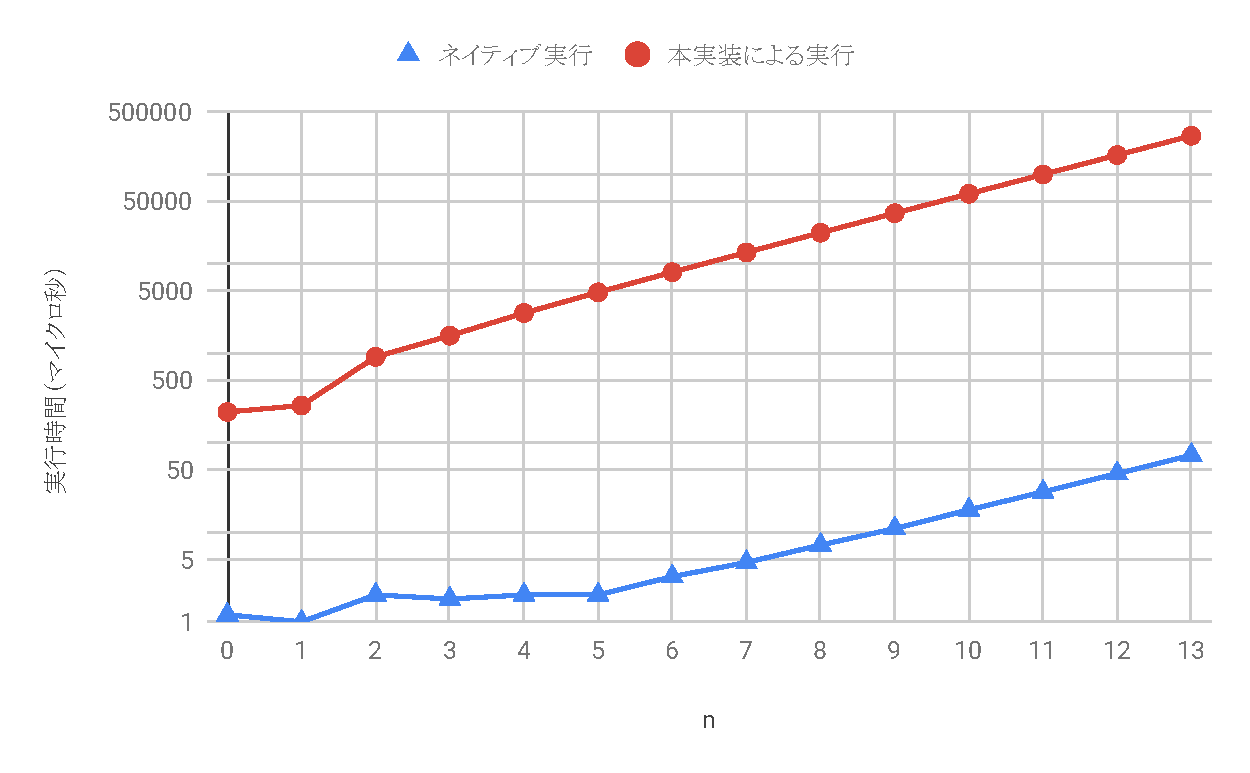
\includegraphics[bb=0 0 600 370,width=10cm]{img/fib_time.pdf}
    \end{center}
  % \end{minipage}
  \end{figure}
  \begin{figure}[htbp]
  % \begin{minipage}{0.5\hsize}
    \caption{実行時間の変化の割合}
    \label{fig:fib_time_diff}
    \begin{center}
      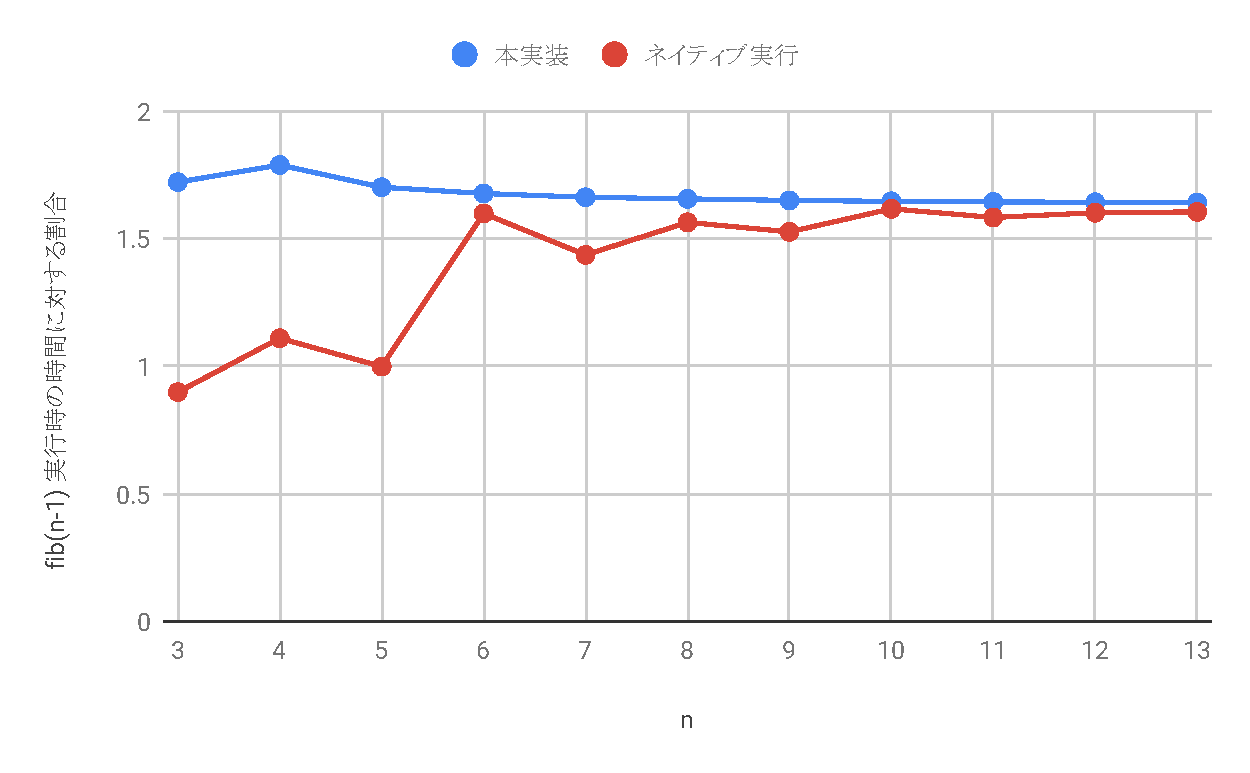
\includegraphics[bb=0 0 600 370,width=10cm]{img/fib_time_diff.pdf}
    \end{center}
  % \end{minipage}
\end{figure}

\section{メモリフットプリント}

また、同プログラムについて、メモリフットプリントとしてヒープ領域に確保されるメモリの最大量を計測した。

FreeRTOSがAPIとして提供する\verb|xPortGetMinimumEverFreeHeapSize|関数は、起動以降一度も確保されていないヒープ領域の最小のサイズを返す。
すなわち、この値の減少分が、処理に必要なメモリフットプリントの増加分と言える。
そこで、モジュールのインスタンス化直後にこの関数で計測した値を0とし、フィボナッチ関数を実行した後の同関数が返す値との差分を取り、関数実行におけるメモリフットプリントとした。

引数\verb|n|を0から13まで変化させた際の、関数実行のメモリフットプリントの推移を図\ref{fig:heap_size}に示す。

\begin{figure}[htbp]
  \caption{メモリフットプリントの推移とその比較}
  \label{fig:heap_size}
  \begin{center}
    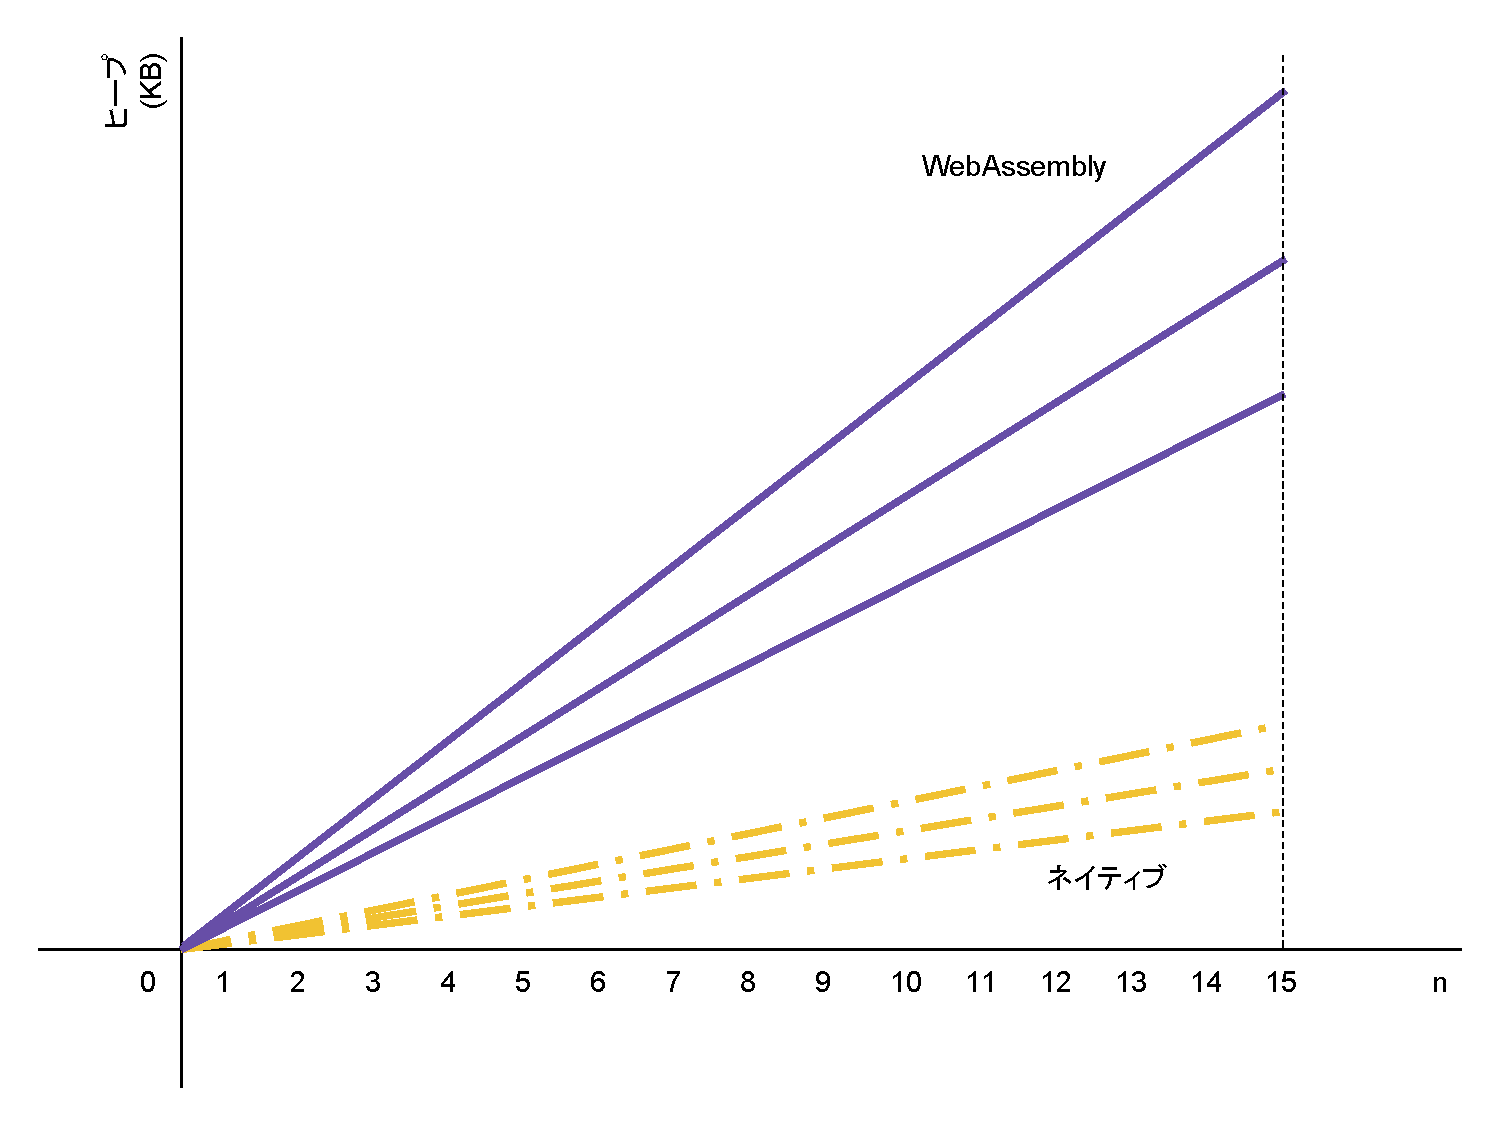
\includegraphics[bb=0 0 600 370,width=10cm]{img/heap_size.pdf}
  \end{center}
\end{figure}

定数を返すのみである$n=0$および$n=1$の時、メモリフットプリントは540バイトで、実行速度と同様に変化はなかった。
再帰的な関数呼び出しが発生する$n=2$以降は、208バイトずつ上昇していった。
これは、WebAssembly実行環境のスタックにおけるメモリ消費であると考えられる。

(分析と考察)

(スタックサイズ150000で27まで計算できた)
